\chapter{Implementation, integration and test plan}
\section{Implementation plan}
The implementation of Data4Help will be done component by component, developing the most critical components first.
The implementation order will be the following:
\begin{enumerate}
\item Data Manager: this is the most important component of the system, since it is the one that handles the data requests from third parties and translate this requests in queries for the DBMS. 
This is also the component that creates a direct communication between the third party web application and the individual application, when the third party sends an individual data request
\item Data Collector: this component is the one that uploads the received data to the database. The Data Collector is also critical, all the individual's data will pass through it while using Data4Help. Furthermore, it is the one that has to interacts with the map external service.
\item Automated SOS: this component is the one that handles all the functionalities linked to the AutomatedSOS service such as the subscription, the vital parameters threshold check and the ambulance call. Of course, to call the ambulance, it has to interact with the ambulance external service.
\item Login Service: this will be the last server side component to be implemented since it is not related to Data4Help main functionalities.
\item Application: once the server side is ready, the application can be developed. The application will be developed before than the third parties web application because it has some critical aspects like the wearable pairing and the AutomatedSOS subscriptio.
\item Web Application: this will be the last component to be implemented.
\end{enumerate}

\section{Integration and testing} 
\subsection{Entry criteria}
The integration and testing plan will follow the implementation plan using a bottom up approach: each component will be fully tested as soon as it is finished and will be integrated with other related components, creating a subcomponent of the whole system that will be again tested to make sure everything works fine.
More precisely:
\begin{itemize}
\item Data Manager: this component will be tested by simulating third parties data requests.
\item Data Collector: this component will be tested by simulating individual's data upload. Once the Data Collector is proved to be fully working, it is integrated with the Data Manager, and a new testing phase that checks if the data uploaded through the Data Collector to the DBMS can be used by the Data Manager to satisfy third parties requests.
\item AutomatedSOS: this component will be tested by checking if the ambulance is called by analyzing simulated vital data. Once it is tested, it will be integrated with the Data Collector, and the interaction between the two components will be tested to see if the data delivered to the Data Collector is correctly analyzed by AutomatedSOS.
\item Login Service: this component will be tested with simulated data, and will be integrated with the Data Manager service to see if a simulated third party individual request can refer to an individual account added through the Login Service.
\end{itemize}



\subsection{Components to be integrated}
In our system, components must be integrated with the DBMS, with external services, among them and finally the clients must be integrated with the business logic server.

\subsubsection{Components to be integrated with the DBMS}
All the components of the server interact with the DBMS, therefore it is necessary perform integration testing between them and the DBMS in order to be sure that the components update correctly the DB and/or their queries are well formulated and the results correctly interpreted.

\begin{figure}[H]
\centering
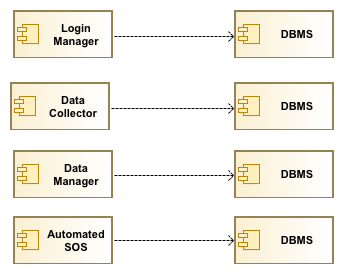
\includegraphics[scale=0.7]{resources/uml/integration/dbms}
\caption{Components to be integrated with the DBMS}
\end{figure}


\subsubsection{Components to be integrated with external services}


\begin{figure}[H]
\centering
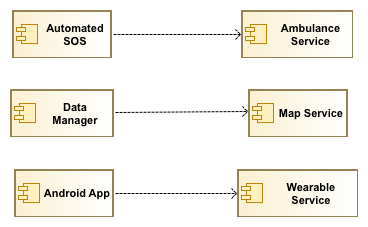
\includegraphics[scale=0.7]{resources/uml/integration/external}
\caption{Components to be integrated with external services}
\end{figure}



\subsubsection{Components to be integrated within the server}
Only the Data Collector and the Automated SOS components directly interact inside the server.
Their integration test aims to guarantee that vital data of the SOS service subscriber, and only that data, is forwarded from the Data Collector to the Automated SOS.

\begin{figure}[H]
\centering
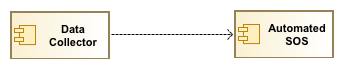
\includegraphics[scale=0.7]{resources/uml/integration/server}
\caption{Components to be integrated within the server}
\end{figure}


\subsubsection{Integration clients/server}
Finally, the interaction between the clients and the server must be also tested.
These tests must assure that the communications are correctly carried on and all the various interfaces must be checked.
This will be the last step of the integration testing because the TrackMe server is seen as a single component, therefore its subcomponents must be already integrated and tested.

\begin{figure}[H]
\centering
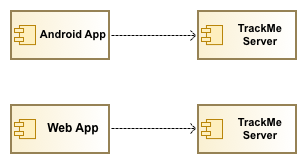
\includegraphics[scale=0.7]{resources/uml/integration/clients}
\caption{Integration clients/server}
\end{figure}



